\subsection{Round 1 Problems}

Solutions can be found in Section~\ref{S::2022-O-1}.

\begin{enumerate}
    \hyperrefitem[Q::2022-O-1-1] If $S = \displaystyle\sum_{k = -2021}^{2021} \frac{1}{10^k + 1}$, find $\floor{2S}$.
    \hyperrefitem[Q::2022-O-1-2] All the positive integers $1, 2, 3, 4, \cdots,$ are grouped in the following way: $G_1 = \bc{1, 2}$, $G_2 = \bc{3, 4, 5, 6}$, $G_3 = \bc{7, 8, 9, 10, 11, 12, 13, 14}$, that is, the set $G_n$ contains the next $2^n$ positive integers listed in ascending order after the set $G_{n-1}$, $n > 1$. If $S$ is the sum of all the positive integers from $G_1$ to $G_8$, find $\floor{\frac{S}{100}}$.
    \hyperrefitem[Q::2022-O-1-3] A sequence of one hundred positive integers $x_1, x_2, x_3, \cdots, x_{100}$ are such that \[(x_1)^2 + (2x_2)^2 + (3x_3)^2 + (4x_4)^2 + \cdots + (100x_{100})^2 = 338350.\] Find the largest possible value of $x_1 + x_2 + x_3 + \cdots + x_{100}$.
    \hyperrefitem[Q::2022-O-1-4] Let $a$ and $b$ be two real numbers satisfying $a < b$, and such that for each real number $m$ satisfying $a < m < b$, the circle $x^2 + (y-m)^2 = 25$ meets the parabola $4y = x^2$ at four distinct points in the Cartesian plane. Let $S$ be the maximum possible value of $b-a$. Find $\floor{4S}$.
    \hyperrefitem[Q::2022-O-1-5] Let $P$ be a point within a rectangle $ABCD$ such that $PA = 10$, $PB = 14$ and $PD = 5$, as shown below. Find $\floor{PC}$.
    
    \begin{center}
        \begin{tikzpicture}[scale=0.7]
            \coordinate[label=above left:$A$] (A) at (0, 5);
            \coordinate[label=below left:$B$] (B) at (0, 0);
            \coordinate[label=below right:$C$] (C) at (10, 0);
            \coordinate[label=above right:$D$] (D) at (10, 5);
            \coordinate[label=below right:$P$] (P) at (7, 3);

            \draw (A) -- (B);
            \draw (B) -- (C);
            \draw (C) -- (D);
            \draw (D) -- (A);
            \draw (A) -- (P);
            \draw (D) -- (P);
            \draw (B) -- (P);
        
            \node[anchor=north east] at ($(A)!0.5!(P)$) {10};
            \node[anchor=north west] at ($(D)!0.5!(P)$) {5};
            \node[anchor=north west] at ($(B)!0.5!(P)$) {14};
        \end{tikzpicture}
    \end{center}
    \hyperrefitem[Q::2022-O-1-6] In the diagram below, the rectangle $ABCD$ has area 180 and both triangles $ABE$ and $ADF$ have areas 60. Find the area of triangle $AEF$.

    \begin{center}
        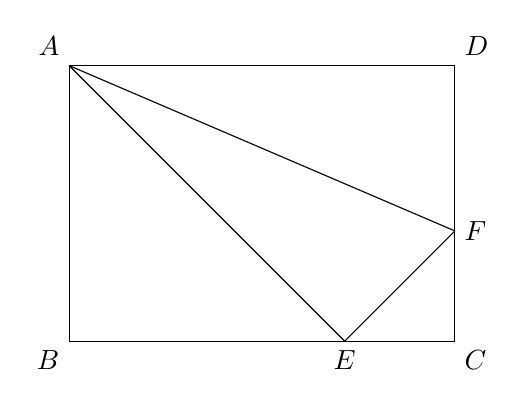
\begin{tikzpicture}[scale=0.7]
            \coordinate[label=above left:$A$] (A) at (0, 5);
            \coordinate[label=below left:$B$] (B) at (0, 0);
            \coordinate[label=below right:$C$] (C) at (7, 0);
            \coordinate[label=above right:$D$] (D) at (7, 5);
            \coordinate[label=below:$E$] (E) at (5, 0);
            \coordinate[label=right:$F$] (F) at (7, 2);

            \draw (A) -- (B);
            \draw (B) -- (C);
            \draw (C) -- (D);
            \draw (D) -- (A);
            \draw (A) -- (E);
            \draw (E) -- (F);
            \draw (A) -- (F);
        \end{tikzpicture}
    \end{center}
    \hyperrefitem[Q::2022-O-1-7] A tetrahedron in $\RR^3$ has one vertex at the origin $O$ and other vertices at the points $A(6, 0, 0)$, $B(4, 2, 4)$ and $C(3, 2, 6)$. If $x$ is the height of the tetrahedron from $O$ to the plane $ABC$, find $\floor{5x^2}$.
    \hyperrefitem[Q::2022-O-1-8] Let $x$ and $y$ be real numbers such that $(x-2)^2 + (y-3)^2 = 4$. If $S$ is the largest possible value of $x^2 + y^2$, find $\floor{(S-17)^2}$.
    \hyperrefitem[Q::2022-O-1-9] Let $S$ be the maximum value of $w^3 - 3w$ subject to the condition that $w^4 + 9 \leq 10w^2$. Find $\floor{S}$.
    \hyperrefitem[Q::2022-O-1-10] In the quadrilateral $ABCD$ below, it is given that $AB = BC = CD$ and $\angle ABC = 80\deg$ and $\angle BCD = 160 \deg$. Suppose $\angle ADC = x\deg$. Find the value of $x$.

    \begin{center}
        \begin{tikzpicture}[scale=0.7]
            \coordinate[label=left:$A$] (A) at (0, 0);
            \coordinate[label=left:$B$] (B) at (0.7, 3);
            \coordinate[label=right:$C$] (C) at (3.5, 2.5);
            \coordinate[label=right:$D$] (D) at (5, 0);

            \draw (A) -- (B);
            \draw (B) -- (C);
            \draw (C) -- (D);
            \draw (D) -- (A);
        \end{tikzpicture}
    \end{center}
    \hyperrefitem[Q::2022-O-1-11] Let $a$, $b$, $c$ be integers with $ab + c = 49$ and $a + bc = 50$. Find the largest possible value of $abc$.
    \hyperrefitem[Q::2022-O-1-12] Find the largest possible value of $\abs a + \abs b$, where $a$ and $b$ are coprime integers (i.e., $a$ and $b$ are integers which have no common factors larger than 1) such that $\frac{a}{b}$ is a solution of the equation below: \[\sqrt{4x + 5 - 4\sqrt{x+1}} + \sqrt{x+2 - 2\sqrt{x+1}} = 1.\]
    \hyperrefitem[Q::2022-O-1-13] Let $S$ be the set of real solutions $(x, y, z)$ of the following system of equations: \[\left\{
        \begin{aligned}
            \frac{4x^2}{1 + 4x^2} = y,\\
            \frac{4y^2}{1 + 4y^2} = z,\\
            \frac{4z^2}{1 + 4z^2} = x.
        \end{aligned}\right.\] For each $(x, y, z) \in S$, define $m(x, y, z) = 2000(\abs x + \abs y + \abs z)$. Determine the maximum value of $m(x, y, z)$ over all $(x, y, z) \in S$.
    \hyperrefitem[Q::2022-O-1-14] Assume that $t$ is a positive solution to the equation \[t = \sqrt{1 + \sqrt{1 + \sqrt{1 + \sqrt{1 + t}}}}.\] Determine the value of $t^4 - t^3 - t + 10$.
    \hyperrefitem[Q::2022-O-1-15] In the triangle $ABC$ shown in the diagram below, the external angle bisectors of $\angle B$ and $\angle C$ meet at the point $D$. The tangent from $D$ to the incircle $\o$ of the triangle $ABC$ touches $\o$ at $E$, where $E$ and $B$ are on the same side of the line $AD$. Suppose $\angle BEC = 112\deg$. Find the size of $\angle A$ in degrees.

    \begin{center}
        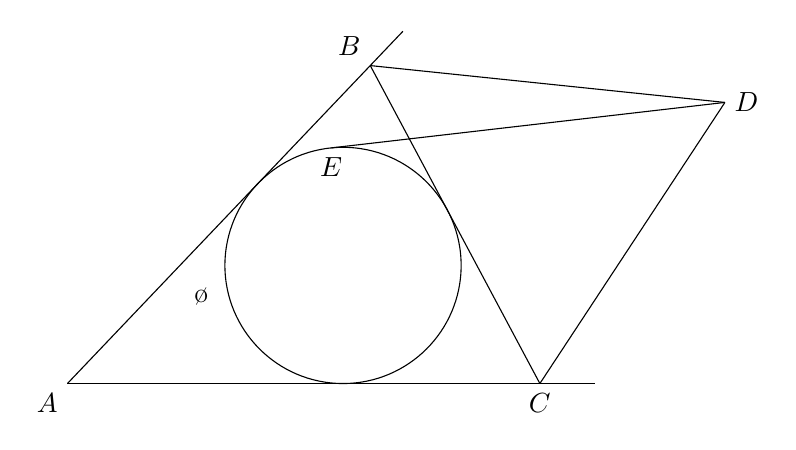
\begin{tikzpicture}
            \coordinate[label=below left:$A$] (A) at (0, 0);
            \coordinate[label=above left:$B$] (B) at (3.846, 4.038);
            \coordinate[label=below:$C$] (C) at (6, 0);
            \coordinate[label=right:$D$] (D) at (8.35, 3.57);
            \coordinate[label=below:$E$] (E) at (3.34871, 2.9923);

            \draw (3.5, 1.5) circle[radius=1.5];

            \draw (A) -- (4.26, 4.473);
            \draw (B) -- (C);
            \draw (6.7, 0) -- (A);
            
            \draw (D) -- (E);
            \draw (B) -- (D);
            \draw (C) -- (D);

            \node at (1.7, 1.1) {$\o$};
        \end{tikzpicture}
    \end{center}
    \hyperrefitem[Q::2022-O-1-16] Find the largest integer $n$ such that $n^2 + 5n - 9486 = 10s(n)$, where $s(n)$ is the product of all digits of $n$ in the decimal representation of $n$.
    
    (For example, $s(481) = 4 \times 8 \times 1 = 32.$)
    \hyperrefitem[Q::2022-O-1-17] Find the number of integer solutions to the equation $19x + 93y = 4xy$.
    \hyperrefitem[Q::2022-O-1-18] Find the number of integer solutions to the equation $x_1 + x_2 - x_3 = 20$ with $x_1 \geq x_2 \geq x_3 \geq 0$.
    \hyperrefitem[Q::2022-O-1-19] In the diagram below, $E$ is a point outside a square $ABCD$ such that $CE$ is parallel to $BD$, $BE = BD$, and $BE$ intersects $CD$ at $H$. Given $BE = \sqrt6 + \sqrt2$, find the length of $DH$.

    \begin{center}
        \begin{tikzpicture}[scale=0.6]
            \coordinate[label=above left:$A$] (A) at (0, 5);
            \coordinate[label=below left:$B$] (B) at (0, 0);
            \coordinate[label=below right:$C$] (C) at (5, 0);
            \coordinate[label=above right:$D$] (D) at (5, 5);
            \coordinate[label=right:$E$] (E) at (6.83, 1.83);
            \coordinate[label=above left:$H$] (H) at (5, 1.34);
            
            \draw (A) -- (B);
            \draw (B) -- (C);
            \draw (C) -- (D);
            \draw (D) -- (A);
            \draw[->-=0.5] (B) -- (D);
            \draw (B) -- (E);
            \draw[->-=0.5] (C) -- (E);
        \end{tikzpicture}
    \end{center}
    \hyperrefitem[Q::2022-O-1-20] The diagram below shows the region $R = \bc{(x, y) \in \RR^2 | y \geq \frac12 x^2}$ on the $xy$-plane bounded by the parabola $y = \frac12 x^2$. Let $C_1$ be the largest circle lying inside $R$ with its lowest point at the origin. Let $C_2$ be the largest circle lying inside $R$ and resting on top of $C_1$. Find the sum of radii of $C_1$ and $C_2$.
    
    \begin{center}
        \begin{tikzpicture}[scale=0.7]
            \begin{axis}[
                domain = -5:5,
                ymax=8,
                axis line style={draw=none},
                tick style={draw=none},
                xticklabel = \empty,
                yticklabel = \empty,
                ]
                \addplot[black] {0.5 * x^2};
    
                \draw (0, 1) circle[radius=1];
                \draw (0, 5) circle[radius=3];
            \end{axis}
        \end{tikzpicture}
    \end{center}
    \hyperrefitem[Q::2022-O-1-21] Find the smallest positive integer $x$ such that $3x^2 + x = 4y^2 + y$ for some positive integer $y$.
    \hyperrefitem[Q::2022-O-1-22] A group of students participates in some sports activities among 6 different types of sports. It is known that for each sport activity there are exactly 100 students in the group participating in it; and the union of all the sports activities participated by any two students is NOT the entire set of 6 sports activities. Determine the minimum number of students in the group.
    \hyperrefitem[Q::2022-O-1-23] Let $p$ and $q$ be positive prime integers such that $p^3 - 5p^2 - 18p = q^9 - 7q$. Determine the smallest value of $p$.
    \hyperrefitem[Q::2022-O-1-24] Given that $a$, $b$, $c$ are positive real numbers such that $a + b + c = 9$, find the maximum value of $a^2 b^3 c^4$.
    \hyperrefitem[Q::2022-O-1-25] Let $\RR^+$ be the set of all positive real numbers. Let $f : \RR^+ \to \RR^+$ be a function satisfying \[xy f(x) \big(f(y) - f(yf(x))\big) = 1\] for all $x, y \in \RR^+$. Find $f(\frac1{2022})$.
\end{enumerate}